% !TEX root = ../thesis.tex
\section{Introduction}
Large language models are typically discussed through the lens of autoregressive decoding, where tokens are generated left-to-right one step at a time. Diffusion language models instead refine a partially masked sequence through iterative denoising, making them a fundamentally different candidate for reasoning and planning \cite{austin2021structured,nie2025llada,ye2025dream}.

This thesis addresses the registered question directly: can chain-of-thought reasoning be rethought through diffusion language models, and if so under what evaluation protocol? The empirical comparison covers two diffusion families (LLaDA-8B and Dream-v0-7B) and two autoregressive families (Qwen2.5-7B and Llama-3.1-8B) across GSM8K, Countdown-cd4, and Trip Planning under both deterministic and stochastic pass@k evaluation \cite{nie2025llada,ye2025dream,qwen2024qwen25,grattafiori2024llama,cobbe2021gsm8k,xie2024travelplanner,chen2021humaneval}.

The current milestone-derived draft has three central contributions. First, diffusion checkpoints are strongest on deterministic or pass@1 planning settings, but autoregressive models overtake at larger k. Second, per-question Pearson correlations show that failure-mode alignment is more strongly organized by generation paradigm than by shared pretrained architecture in key settings. Third, prompt sensitivity differs by paradigm: diffusion models are much stronger at zero-shot GSM8K, whereas autoregressive models benefit more from few-shot examples.

\subsection{Thesis Roadmap}
The thesis is organized around the following chapter-level story, retained from the Milestone 2 outline:
\begin{enumerate}[leftmargin=*]
    \item \textbf{Introduction}: motivate the thesis question and explain why diffusion generation is a meaningful alternative to autoregressive decoding.
    \item \textbf{Related Work}: review discrete diffusion language modeling, open autoregressive baselines, reasoning benchmarks, planning benchmarks, and pass@k evaluation.
    \item \textbf{Methodology}: define benchmarks, checkpoints, prompt modes, inference backends, answer extraction, deterministic versus stochastic evaluation, and the per-question correlation protocol.
    \item \textbf{Results}: present deterministic planning, pass@k ranking reversal, GSM8K prompt/few-shot sensitivity, Trip Planning generalization, hyperparameter analysis, and per-question correlation analysis.
    \item \textbf{Discussion}: interpret why diffusion models have high pass@1 but slower pass@k growth, why autoregressive models scale more strongly with sampling, and why the two paradigms appear complementary.
    \item \textbf{Conclusion and Future Work}: answer the question of which paradigm is better and outline next steps.
\end{enumerate}

\section{Related Work}
The diffusion side of this thesis builds on structured denoising diffusion models in discrete state spaces and on recent large language diffusion systems such as LLaDA and Dream 7B \cite{austin2021structured,nie2025llada,ye2025dream}. These works make token-level denoising a viable large-scale alternative to autoregressive decoding and motivate the central comparison in this thesis.

The autoregressive baselines are intentionally strong open checkpoints at a similar parameter scale. Qwen2.5 and Llama 3.1 provide both base and instruction-tuned variants and serve as practical reference systems for reasoning and planning tasks \cite{qwen2024qwen25,grattafiori2024llama}. On the evaluation side, GSM8K remains a standard benchmark for multi-step mathematical reasoning, TravelPlanner provides a realistic planning benchmark, and the pass@k estimator follows the evaluation protocol popularized in HumanEval \cite{cobbe2021gsm8k,xie2024travelplanner,chen2021humaneval}.

Because inference speed is part of the practical trade-off, this draft also distinguishes fast-dLLM from slower dLLM baselines on the diffusion side and vLLM with PagedAttention on the autoregressive side \cite{kwon2023pagedattention}. This is important for interpreting both deterministic parity checks and the feasibility of large pass@k sweeps.

\section{Methodology}
The methodology chapter is organized around a single evaluation pipeline so that model-family differences can be interpreted under controlled prompts, answer extraction, and reporting. The same benchmarks, prompt constructions, and aggregation rules are reused across all four model families to keep the comparison focused on the generation paradigm rather than on incompatible tooling choices.

\subsection{Benchmark Suite and Experimental Role}
Table~\ref{tab:benchmarks} summarizes the benchmark suite and its role in the thesis narrative.

\begin{table*}[!t]
\caption{Benchmark suite and experimental role in the thesis narrative.}
\label{tab:benchmarks}
\centering
\footnotesize
\begin{tabularx}{\textwidth}{L{2.35cm} Y Y Y}
\toprule
\textbf{Component} & \textbf{Role in the Thesis} & \textbf{Evaluation Mode} & \textbf{Notes} \\
\midrule
GSM8K & Reasoning sanity check and prompt/few-shot sensitivity benchmark & Deterministic and pass@k; base and instruct settings & Near-saturated at 7--8B scale, but informative for prompt sensitivity \\
Countdown-cd4 & Core arithmetic planning benchmark and central ranking-reversal evidence & Deterministic validation plus pass@k ($n=128$) & Main benchmark for the pass@k crossover narrative \\
Trip Planning & Structured natural-language planning benchmark & Deterministic comparison plus pass@k ($n=64$) & Tests whether Countdown patterns generalize beyond arithmetic planning \\
Per-question correlation analysis & Novel analysis of failure-mode alignment & Pearson $r$ on per-question accuracy vectors & 128 samples/model on Countdown and GSM8K; 64 on Trip Planning \\
\bottomrule
\end{tabularx}
\end{table*}

\subsection{Model Families and Inference Backends}
Table~\ref{tab:model-families} lists the model families and inference backends used in Milestone 2.

\begin{table}[!t]
\caption{Model families and inference backends used in Milestone 2.}
\label{tab:model-families}
\centering
\footnotesize
\begin{tabularx}{\columnwidth}{L{1.1cm} Y Y C{0.8cm} Y}
\toprule
\textbf{Family} & \textbf{Base} & \textbf{Instruct} & \textbf{Params} & \textbf{Type} \\
\midrule
LLaDA & GSAI-ML/LLaDA-8B-Base & GSAI-ML/LLaDA-8B-Instruct & 8B & Diffusion (masked) \\
Dream & Dream-org/Dream-v0-Base-7B & Dream-org/Dream-v0-Instruct-7B & 7B & Diffusion (masked, Qwen2.5 backbone) \\
Qwen & Qwen/Qwen2.5-7B & Qwen/Qwen2.5-7B-Instruct & 7B & Autoregressive \\
Llama & meta-llama/Llama-3.1-8B & meta-llama/Llama-3.1-8B-Instruct & 8B & Autoregressive \\
\bottomrule
\end{tabularx}
\end{table}

\subsection{Shared Evaluation Pipeline}
Figure~\ref{fig:pipeline} summarizes the shared evaluation pipeline used for all diffusion and autoregressive experiments.

\begin{figure*}[!t]
\centering
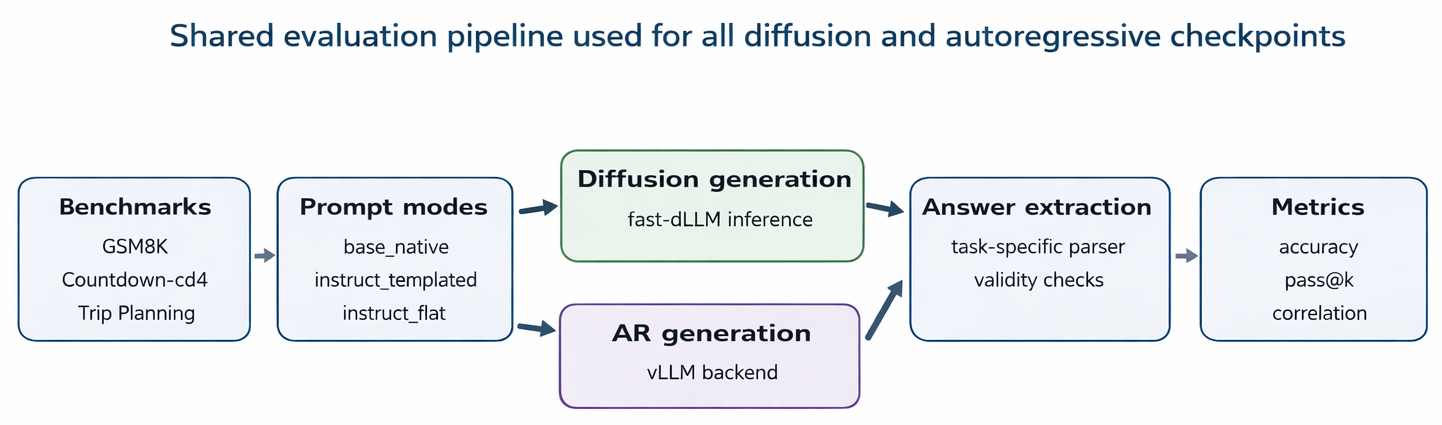
\includegraphics[width=0.98\textwidth]{images/eval_pipeline_ar_vs_dllm.png}
\caption{Shared evaluation pipeline for diffusion and autoregressive experiments. The same benchmark definitions, prompt modes, generation stage, answer extraction, and metrics are used to support comparable analysis across all four model families.}
\label{fig:pipeline}
\end{figure*}

The methodological choices retained in this draft are as follows:
\begin{itemize}[leftmargin=*]
    \item \textbf{Prompt modes}: \texttt{base\_native}, \texttt{instruct\_templated}, and \texttt{instruct\_flat}. The templated instruct setting is the default instruct evaluation; \texttt{instruct\_flat} is an explicit prompt-format ablation.
    \item \textbf{Evaluation modes}: deterministic accuracy uses temperature $=0$ and \texttt{n\_samples}$=1$; pass@k uses temperature $=0.7$ with $n=16$, $64$, or $128$ depending on benchmark and setup.
    \item \textbf{Inference provenance}: all main dLLM comparisons use fast-dLLM, all main autoregressive comparisons use vLLM, and standard dLLM / AR-HF runs are retained only for targeted deterministic validation.
    \item \textbf{Correlation protocol}: per-question Pearson correlations are computed from question-level accuracy vectors using 128 samples/model on Countdown and GSM8K and 64 samples/model on Trip Planning.
\end{itemize}

\section{Results}
The figures and tables in this section provide the milestone-ready empirical evidence supporting the thesis story. Pass@k result grids are described directly from the milestone values, while compact deterministic/pass@1 tables preserve the single-shot results in a format that is easy to scan.

\subsection{GSM8K: Reasoning Sanity Check and Prompt/Few-Shot Sensitivity}
GSM8K is the least decisive benchmark for the final ranking because all models approach saturation at larger $k$. Its most useful role in this draft is therefore diagnostic: it shows that diffusion models are much stronger at zero-shot instruct prompting, whereas autoregressive models benefit more from few-shot examples and can catch up or overtake under stronger prompting.

\begin{table}[!t]
\caption{GSM8K deterministic/pass@1 summary across base and instruct configurations.}
\label{tab:gsm8k-pass1}
\centering
\footnotesize
\begin{tabular}{L{2.35cm}C{1.1cm}C{1.1cm}C{1.1cm}C{1.1cm}}
\toprule
\textbf{Condition} & \textbf{LLaDA} & \textbf{Dream} & \textbf{Qwen} & \textbf{Llama} \\
\midrule
Base, 0-shot ($n=128$) & 63.14\% & 72.39\% & 70.93\% & 14.33\% \\
Base, 4-shot ($n=16$) & 66.48\% & 71.34\% & 72.27\% & 14.53\% \\
Instruct, 0-shot ($n=16$) & 74.85\% & 73.39\% & 53.37\% & 48.78\% \\
Instruct, 4-shot ($n=16$) & 77.47\% & 76.15\% & 78.88\% & 78.20\% \\
Instruct templated, 4-shot ($n=128$) & 75.57\% & 76.15\% & 79.77\% & 78.22\% \\
Instruct flat, 4-shot ($n=128$) & 76.90\% & 70.93\% & 73.83\% & 21.05\% \\
\bottomrule
\end{tabular}
\end{table}

\begin{figure*}[!t]
\centering
\figplaceholder{GSM8K pass@k curves across base and instruct settings. Replace with the four-panel plot showing base 0-shot, base 4-shot, instruct 0-shot, and instruct 4-shot settings.}{1.85in}
\caption{GSM8K pass@k curves across base and instruct settings. Panels A--D show that GSM8K is near-saturated at 7--8B scale, but they also reveal a clear paradigm difference in prompt sensitivity: diffusion instruct models start much higher at 0-shot, whereas autoregressive instruct models gain more from 4-shot prompting. Source note retained from the milestone draft: redrawn from \texttt{MILESTONE\_2\_DRAFT.md} Sections 3.1, 3.2, 3.4, and 3.5.}
\label{fig:gsm8k-panels}
\end{figure*}

\begin{figure*}[!t]
\centering
\figplaceholder{GSM8K instruct prompt-format sensitivity at $n=128$. Replace with the templated-vs-flat prompt comparison plot.}{1.65in}
\caption{GSM8K instruct prompt-format sensitivity at $n=128$. Templated prompts (solid) and flat prompts (dashed) behave similarly for most checkpoints, but Llama-3.1-8B-Instruct drops from 78.22\% to 21.05\% at pass@1 when the prompt is flattened.}
\label{fig:gsm8k-prompt-format}
\end{figure*}

The exact pass@1 values make the paradigm difference especially clear. At 0-shot instruct, LLaDA-8B-Instruct reaches 74.85\% and Dream-v0-Instruct-7B reaches 73.39\%, versus 53.37\% for Qwen2.5-7B-Instruct and 48.78\% for Llama-3.1-8B-Instruct. At 4-shot instruct, the gap closes: Qwen rises to 78.88\% and Llama to 78.20\%, while LLaDA reaches 77.47\% and Dream 76.15\%. This supports the thesis claim that autoregressive models depend more strongly on in-context examples, whereas diffusion language models show stronger zero-shot generalization on GSM8K.

\subsection{Countdown-cd4: Core Planning Benchmark}
Countdown is the central benchmark in this draft because it makes the evaluation-protocol story unambiguous. Deterministically, diffusion models are much stronger; under pass@k, autoregressive models scale much more steeply and reverse the ranking at larger $k$.

\begin{table*}[!t]
\caption{Countdown deterministic comparison.}
\label{tab:countdown-deterministic}
\centering
\footnotesize
\begin{tabular}{L{1.8cm}L{1.3cm}C{1.25cm}C{1.2cm}C{1.25cm}C{1.2cm}C{1.1cm}}
\toprule
\textbf{Model} & \textbf{Method} & \textbf{Acc (bs=1)} & \textbf{Time (bs=1)} & \textbf{Acc (bs=8)} & \textbf{Time (bs=8)} & \textbf{Speedup} \\
\midrule
LLaDA-Base & Fast-dLLM & 13.7\% & 16m 9s & 14.5\% & 5m 19s & 3.03$\times$ \\
LLaDA-Base & dLLM & 15.4\% & 25m 31s & 14.7\% & 30m 1s & 0.85$\times$ \\
Dream-Base & Fast-dLLM & 14.4\% & 15m 46s & 14.1\% & 6m 46s & 2.33$\times$ \\
Dream-Base & dLLM & 14.6\% & 23m 39s & 14.3\% & 18m 35s & 1.27$\times$ \\
Qwen-Base & vLLM & 6.0\% & 6m 35s & 6.0\% & 51.6s & 7.65$\times$ \\
Qwen-Base & AR & 6.0\% & 13m 46s & 6.0\% & 2m 36s & 5.31$\times$ \\
LLaDA-Inst & Fast-dLLM & 1.5\% & 16m 0s & 1.9\% & 5m 38s & 2.84$\times$ \\
LLaDA-Inst & dLLM & 1.9\% & 25m 56s & 1.8\% & 30m 50s & 0.84$\times$ \\
Dream-Inst & Fast-dLLM & 7.5\% & 12m 16s & 7.9\% & 6m 4s & 2.02$\times$ \\
Dream-Inst & dLLM & 3.5\% & 23m 43s & 3.4\% & 19m 0s & 1.25$\times$ \\
Qwen-Inst & vLLM & 2.6\% & 6m 33s & 2.8\% & 51.9s & 7.58$\times$ \\
Qwen-Inst & AR & 1.0\% & 14m 2s & 0.9\% & 2m 43s & 5.16$\times$ \\
\bottomrule
\end{tabular}
\end{table*}

\begin{table}[!t]
\caption{Countdown pass@1 summary across base, instruct-templated, and instruct-flat settings.}
\label{tab:countdown-pass1}
\centering
\footnotesize
\begin{tabular}{L{2.1cm}C{1.0cm}C{1.0cm}C{1.0cm}C{1.0cm}}
\toprule
\textbf{Setting} & \textbf{LLaDA} & \textbf{Dream} & \textbf{Qwen} & \textbf{Llama} \\
\midrule
Base pass@1 ($n=128$) & 14.29\% & 11.30\% & 4.04\% & 2.70\% \\
Instruct templated pass@1 ($n=128$) & 2.41\% & 9.15\% & 7.84\% & 5.78\% \\
Instruct flat pass@1 (earlier smaller run) & 2.84\% & 1.81\% & 1.05\% & 4.99\% \\
\bottomrule
\end{tabular}
\end{table}

\begin{figure*}[!t]
\centering
\figplaceholder{Countdown-cd4 base-model pass@k crossover (R1). Replace with the crossover plot showing diffusion models starting higher at low $k$ and autoregressive models overtaking around $k=8$--$16$.}{1.8in}
\caption{Countdown-cd4 base-model pass@k crossover (R1). Diffusion models start higher at low $k$, but autoregressive models grow more steeply and overtake around $k=8$--$16$, making this the central ranking-reversal figure of the thesis.}
\label{fig:countdown-base-crossover}
\end{figure*}

\begin{figure*}[!t]
\centering
\figplaceholder{Countdown-cd4 instruct-model pass@k under templated prompting. Replace with the instruct pass@k plot.}{1.8in}
\caption{Countdown-cd4 instruct-model pass@k under templated prompting. Dream-v0-Instruct-7B remains competitive, Llama-3.1-8B-Instruct becomes the strongest high-$k$ model, and LLaDA-8B-Instruct remains near-collapsed throughout the curve.}
\label{fig:countdown-instruct-passk}
\end{figure*}

\begin{figure*}[!t]
\centering
\figplaceholder{Countdown prompt-mode diagnostic from earlier smaller instruct runs. Replace with the templated-vs-flat prompt comparison plot.}{1.65in}
\caption{Countdown prompt-mode diagnostic from earlier smaller instruct runs. Prompt formatting changes Dream and Qwen substantially, but it barely changes the already-strong Llama-Instruct curve and does not rescue LLaDA-Instruct.}
\label{fig:countdown-prompt-diagnostic}
\end{figure*}

The exact base-model ordering is the key result. At pass@1, LLaDA (14.29\%) $>$ Dream (11.30\%) $>$ Qwen (4.04\%) $>$ Llama (2.70\%), so diffusion models dominate. At pass@128, the ranking reverses to Qwen (51.31\%) $>$ Llama (49.50\%) $>$ Dream (37.60\%) $>$ LLaDA (27.22\%). The crossover occurs around pass@8--16 for Dream versus the autoregressive baselines and around pass@16--32 for LLaDA versus the autoregressive baselines. This is the clearest evidence that diffusion language models concentrate probability mass into a smaller set of strong samples, whereas autoregressive models maintain broader diversity and therefore scale more strongly under pass@k evaluation.

The deterministic table adds the practical runtime story. Fast-dLLM preserves much of the diffusion quality while materially reducing latency relative to standard dLLM, but vLLM remains much faster for the autoregressive checkpoints. In the instruct setting, Dream-Instruct is the only diffusion checkpoint that remains competitive; LLaDA-Instruct reaches only 5.54\% at pass@128 under templated prompting.

\subsection{Trip Planning: Structured Natural-Language Planning}
Trip Planning generalizes the Countdown narrative to a more natural planning benchmark. Dream remains strongest at low-$k$ and deterministic settings, but the flatter autoregressive distributions scale more aggressively under sampling and become strongest at larger $k$, especially for Llama flat prompting.

\begin{table}[!t]
\caption{Trip Planning deterministic comparison.}
\label{tab:trip-deterministic}
\centering
\footnotesize
\begin{tabularx}{\columnwidth}{Y C{1.2cm}}
\toprule
\textbf{Model / Variant} & \textbf{Accuracy} \\
\midrule
Dream-v0-Instruct-7B [bl=256] [dllm] & 15.00\% \\
Dream-v0-Base-7B [bl=256] [dllm] & 14.50\% \\
Dream-v0-Base-7B [bl=32] [fast-dllm] & 13.50\% \\
Dream-v0-Instruct-7B [bl=32] [fast-dllm] & 12.50\% \\
Dream-v0-Instruct-7B [flat] [bl=32] [fast-dllm] & 12.50\% \\
Dream-v0-Base-7B [bl=256] [dllm] & 14.50\% \\
LLaDA-8B-Base [bl=256] [dllm] & 11.50\% \\
Llama-3.1-8B-Instruct [flat] [vllm] & 9.50\% \\
LLaDA-8B-Instruct [bl=256] [dllm] & 8.00\% \\
LLaDA-8B-Base [bl=32] [fast-dllm] & 5.00\% \\
Llama-3.1-8B [vllm] & 4.50\% \\
LLaDA-8B-Instruct [bl=32] [dllm] & 4.50\% \\
Qwen2.5-7B [vllm] & 1.50\% \\
Qwen2.5-7B-Instruct [vllm] & 1.50\% \\
Llama-3.1-8B-Instruct [vllm] & 2.00\% \\
Qwen2.5-7B-Instruct [flat] [vllm] & 2.00\% \\
\bottomrule
\end{tabularx}
\end{table}

\begin{table}[!t]
\caption{Trip Planning pass@1 summary for all stochastic milestone runs.}
\label{tab:trip-pass1}
\centering
\footnotesize
\begin{tabularx}{\columnwidth}{Y C{1.2cm}}
\toprule
\textbf{Model} & \textbf{pass@1} \\
\midrule
Dream-v0-Base-7B [fast-dllm] & 5.44\% \\
Dream-v0-Instruct-7B [fast-dllm] & 5.66\% \\
LLaDA-8B-Base [fast-dllm] & 3.55\% \\
LLaDA-8B-Instruct [fast-dllm] & 1.04\% \\
LLaDA-8B-Instruct [flat] [fast-dllm] & 1.24\% \\
Llama-3.1-8B [vllm] & 2.50\% \\
Llama-3.1-8B-Instruct [vllm] & 1.66\% \\
Llama-3.1-8B-Instruct [flat] [vllm] & 6.00\% \\
Qwen2.5-7B [vllm] & 1.48\% \\
Qwen2.5-7B-Instruct [vllm] & 1.65\% \\
\bottomrule
\end{tabularx}
\end{table}

\begin{figure*}[!t]
\centering
\figplaceholder{Trip Planning pass@k for all Milestone 2 checkpoints. Replace with the full all-model pass@k plot.}{1.85in}
\caption{Trip Planning pass@k for all Milestone 2 checkpoints. Dream-v0-Base-7B leads the standard checkpoints at pass@1, while Llama-3.1-8B-Instruct with flat prompting becomes the strongest high-$k$ curve and reaches 29.50\% at pass@64.}
\label{fig:trip-passk}
\end{figure*}

The pass@k comparison is most easily summarized through growth rates. Dream-v0-Base-7B starts at 5.44\% pass@1 and reaches 22.50\% at pass@64, whereas Llama-3.1-8B-Instruct [flat] starts at 6.00\% and reaches 29.50\% by pass@64. Standard Qwen and Llama base checkpoints start low but scale steadily, while LLaDA-Instruct remains weak even after switching to flat prompts. Together with Countdown, this supports the thesis claim that diffusion models offer stronger single-shot planning quality, while autoregressive models offer stronger search behavior when multiple samples are allowed.

\subsection{Hyperparameter Analysis and the Pivot Away from Tuning}
Before settling on the comparative pass@k story, the project conducted an extensive GSM8K hyperparameter sweep for LLaDA-8B, Dream-7B, and Qwen2.5-7B. The sweep matters because it justifies why the thesis pivots away from \emph{find the single best diffusion-language-model configuration} and toward \emph{compare paradigms under a controlled evaluation protocol}.

\begin{table}[!t]
\caption{Best pass@1 configurations from the GSM8K hyperparameter sweep.}
\label{tab:hyperparams-pass1}
\centering
\footnotesize
\begin{tabular}{L{1.5cm}L{1.5cm}C{1.0cm}C{0.9cm}}
\toprule
\textbf{Model} & \textbf{Best pass@1 Config} & \textbf{pass@1} & \textbf{Time} \\
\midrule
LLaDA-8B & g256\_s256\_b128 & 71.01\% & 14.5 min \\
Dream-7B & g256\_s32\_b32 & 70.66\% & 11.8 min \\
Qwen2.5-7B & g256 (vLLM) & 72.97\% & 5.7 min \\
\bottomrule
\end{tabular}
\end{table}

\begin{figure*}[!t]
\centering
\figplaceholder{Hyperparameter sweep summary: best pass@128 by model and configuration. Replace with the bar chart showing LLaDA-8B, Dream-7B, and Qwen2.5-7B best pass@128 values.}{1.75in}
\caption{Hyperparameter sweep summary for best pass@128 by model and configuration. Even after tuning, the sweep does not produce a single dominant diffusion configuration that would remove the need for a paradigm-level comparison.}
\label{fig:hyperparameter-summary}
\end{figure*}

The main findings retained from the sweep are:
\begin{itemize}[leftmargin=*]
    \item Generation length is the most impactful parameter. Moving from 128 to 256 tokens improves pass@1 by roughly 20--25 percentage points.
    \item Step count shows diminishing returns: 128--256 steps are the useful range, while 32 steps significantly underperform.
    \item Block length has nuanced effects; smaller block lengths such as 32 often improve the quality-versus-latency trade-off.
    \item No single configuration dominates across pass@1, pass@128, and runtime. This motivates the pivot from hyperparameter hunting to controlled comparative pass@k analysis.
\end{itemize}

\subsection{Per-Question Correlation Analysis}
The most novel addition in the revised milestone draft is the per-question correlation analysis. For each question, accuracy is computed as the fraction of correct samples for that model, and Pearson correlation is then measured between model pairs across questions. This turns the comparison from ``which model scores higher on average?'' into ``which models succeed on the same questions?''

\begin{figure*}[!t]
\centering
\figplaceholder{Cross-benchmark summary of within-paradigm and strongest cross-paradigm correlations. Replace with the bar chart summarizing dLLM--dLLM, AR--AR, and strongest cross-paradigm correlations.}{1.75in}
\caption{Cross-benchmark summary of within-paradigm and strongest cross-paradigm correlations. Diffusion models agree most on Countdown Base, autoregressive models agree most on Trip Planning, and GSM8K shows a more mixed pattern.}
\label{fig:correlation-summary}
\end{figure*}

\begin{figure*}[!t]
\centering
\figplaceholder{Placeholder layout for the six interactive HTML comparison views. Replace with screenshots or actual exported comparison views if these are added later.}{1.6in}
\caption{Placeholder layout for the six interactive HTML comparison views (R2). The milestone draft names six HTML files for per-question inspection; this placeholder records their role without fabricating scatter-plot data that are not included in the authoritative milestone draft. Source note retained from the milestone draft: author placeholder based on \texttt{MILESTONE\_2\_DRAFT.md} Section 7.8.}
\label{fig:html-placeholder}
\end{figure*}

\begin{table}[!t]
\caption{Countdown Base per-question correlation matrix.}
\label{tab:countdown-base-corr}
\centering
\footnotesize
\begin{tabular}{L{1.65cm}L{1.15cm}C{0.8cm}C{1.0cm}}
\toprule
\textbf{Model Pair} & \textbf{Type} & \textbf{$r$} & \textbf{$p$-value} \\
\midrule
LLaDA-Base vs Dream-Base & dLLM--dLLM & 0.6382 & $1.4\times10^{-114}$ \\
Qwen-Base vs Llama-Base & AR--AR & 0.6149 & $3.1\times10^{-104}$ \\
Dream-Base vs Qwen-Base & dLLM--AR (shared arch) & 0.5718 & $3.5\times10^{-87}$ \\
LLaDA-Base vs Qwen-Base & dLLM--AR & 0.5342 & $2.8\times10^{-74}$ \\
LLaDA-Base vs Llama-Base & dLLM--AR & 0.4580 & $1.3\times10^{-52}$ \\
Dream-Base vs Llama-Base & dLLM--AR & 0.4432 & $5.6\times10^{-49}$ \\
\bottomrule
\end{tabular}
\end{table}

\begin{table}[!t]
\caption{Countdown Instruct per-question correlation matrix.}
\label{tab:countdown-inst-corr}
\centering
\footnotesize
\begin{tabular}{L{1.65cm}L{1.15cm}C{0.8cm}C{1.0cm}}
\toprule
\textbf{Model Pair} & \textbf{Type} & \textbf{$r$} & \textbf{$p$-value} \\
\midrule
Dream-Inst vs Llama-Inst & dLLM--AR & 0.4345 & $6.1\times10^{-47}$ \\
Dream-Inst vs Qwen-Inst & dLLM--AR & 0.4062 & $1.1\times10^{-40}$ \\
Qwen-Inst vs Llama-Inst & AR--AR & 0.4039 & $3.3\times10^{-40}$ \\
LLaDA-Inst vs Dream-Inst & dLLM--dLLM & 0.1475 & $3.1\times10^{-6}$ \\
LLaDA-Inst vs Llama-Inst & dLLM--AR & 0.1464 & $3.6\times10^{-6}$ \\
LLaDA-Inst vs Qwen-Inst & dLLM--AR & 0.0867 & $6.3\times10^{-3}$ \\
\bottomrule
\end{tabular}
\end{table}

\begin{table}[!t]
\caption{GSM8K Base per-question correlation matrix.}
\label{tab:gsm8k-base-corr}
\centering
\footnotesize
\begin{tabular}{L{1.65cm}L{1.15cm}C{0.8cm}C{1.0cm}}
\toprule
\textbf{Model Pair} & \textbf{Type} & \textbf{$r$} & \textbf{$p$-value} \\
\midrule
LLaDA-Base vs Dream-Base & dLLM--dLLM & 0.6291 & $1.8\times10^{-15}$ \\
Dream-Base vs Qwen-Base & dLLM--AR (shared arch) & 0.6189 & $6.9\times10^{-15}$ \\
LLaDA-Base vs Qwen-Base & dLLM--AR & 0.4907 & $4.1\times10^{-9}$ \\
LLaDA-Base vs Llama-Base & dLLM--AR & 0.4316 & $3.7\times10^{-7}$ \\
Dream-Base vs Llama-Base & dLLM--AR & 0.3510 & $4.9\times10^{-5}$ \\
Qwen-Base vs Llama-Base & AR--AR & 0.3204 & $2.3\times10^{-4}$ \\
\bottomrule
\end{tabular}
\end{table}

\begin{table}[!t]
\caption{GSM8K Instruct per-question correlation matrix.}
\label{tab:gsm8k-inst-corr}
\centering
\footnotesize
\begin{tabular}{L{1.65cm}L{1.15cm}C{0.8cm}C{1.0cm}}
\toprule
\textbf{Model Pair} & \textbf{Type} & \textbf{$r$} & \textbf{$p$-value} \\
\midrule
Qwen-Inst vs Llama-Inst & AR--AR & 0.6638 & $1.4\times10^{-17}$ \\
LLaDA-Inst vs Llama-Inst & dLLM--AR & 0.6550 & $5.0\times10^{-17}$ \\
Dream-Inst vs Llama-Inst & dLLM--AR & 0.6398 & $4.3\times10^{-16}$ \\
LLaDA-Inst vs Dream-Inst & dLLM--dLLM & 0.5671 & $3.0\times10^{-12}$ \\
Dream-Inst vs Qwen-Inst & dLLM--AR (shared arch) & 0.5598 & $6.5\times10^{-12}$ \\
LLaDA-Inst vs Qwen-Inst & dLLM--AR & 0.4847 & $6.8\times10^{-9}$ \\
\bottomrule
\end{tabular}
\end{table}

\begin{table}[!t]
\caption{Trip Planning Base per-question correlation matrix.}
\label{tab:trip-base-corr}
\centering
\footnotesize
\begin{tabular}{L{1.65cm}L{1.15cm}C{0.8cm}C{1.0cm}}
\toprule
\textbf{Model Pair} & \textbf{Type} & \textbf{$r$} & \textbf{$p$-value} \\
\midrule
Qwen-Base vs Llama-Base & AR--AR & 0.7061 & $1.7\times10^{-31}$ \\
LLaDA-Base vs Llama-Base & dLLM--AR & 0.5394 & $1.7\times10^{-16}$ \\
LLaDA-Base vs Qwen-Base & dLLM--AR & 0.5158 & $5.5\times10^{-15}$ \\
Dream-Base vs Qwen-Base & dLLM--AR (shared arch) & 0.4829 & $4.4\times10^{-13}$ \\
Dream-Base vs Llama-Base & dLLM--AR & 0.3629 & $1.3\times10^{-7}$ \\
LLaDA-Base vs Dream-Base & dLLM--dLLM & 0.3451 & $5.6\times10^{-7}$ \\
\bottomrule
\end{tabular}
\end{table}

\begin{table}[!t]
\caption{Trip Planning Instruct per-question correlation matrix.}
\label{tab:trip-inst-corr}
\centering
\footnotesize
\begin{tabular}{L{1.65cm}L{1.15cm}C{0.8cm}C{1.0cm}}
\toprule
\textbf{Model Pair} & \textbf{Type} & \textbf{$r$} & \textbf{$p$-value} \\
\midrule
Qwen-Inst vs Llama-Inst & AR--AR & 0.7190 & $4.1\times10^{-33}$ \\
LLaDA-Inst vs Dream-Inst & dLLM--dLLM & 0.4622 & $5.6\times10^{-12}$ \\
Dream-Inst vs Llama-Inst & dLLM--AR & 0.2484 & $3.9\times10^{-4}$ \\
LLaDA-Inst vs Qwen-Inst & dLLM--AR & 0.2170 & $2.0\times10^{-3}$ \\
LLaDA-Inst vs Llama-Inst & dLLM--AR & 0.1647 & $2.0\times10^{-2}$ \\
Dream-Inst vs Qwen-Inst & dLLM--AR (shared arch) & 0.1572 & $2.6\times10^{-2}$ \\
\bottomrule
\end{tabular}
\end{table}

\begin{table}[!t]
\caption{Summary of within-paradigm and strongest cross-paradigm correlations across benchmark-variant conditions.}
\label{tab:corr-summary-table}
\centering
\footnotesize
\begin{tabular}{L{1.6cm}C{0.9cm}C{0.9cm}L{1.4cm}}
\toprule
\textbf{Benchmark} & \textbf{dLLM--dLLM ($r$)} & \textbf{AR--AR ($r$)} & \textbf{Strongest cross-paradigm ($r$)} \\
\midrule
Countdown Base & 0.638 & 0.615 & Dream--Qwen: 0.572 \\
Countdown Instruct & 0.148$^{*}$ & 0.404 & Dream--Llama: 0.435 \\
Trip Planning Base & 0.345 & 0.706 & LLaDA--Llama: 0.539 \\
Trip Planning Instruct & 0.462 & 0.719 & Dream--Llama: 0.248 \\
GSM8K Base & 0.629 & 0.320 & Dream--Qwen: 0.619 \\
GSM8K Instruct & 0.567 & 0.664 & LLaDA--Llama: 0.655 \\
\bottomrule
\end{tabular}
\end{table}

The main milestone findings from the per-question correlation analysis are:
\begin{itemize}[leftmargin=*]
    \item \textbf{Finding 1}: On Countdown Base, the strongest correlation is between the two diffusion models: LLaDA-Base versus Dream-Base reaches $r=0.6382$, which is higher than Dream-Base versus Qwen-Base at $r=0.5718$ even though Dream shares the Qwen2.5 backbone. This is the strongest evidence that generation paradigm matters more than pretrained weights for failure-mode alignment in this setting.
    \item \textbf{Finding 2}: On Trip Planning, the AR--AR pair is strongest in both Base and Instruct settings. Qwen-Base versus Llama-Base reaches $r=0.7061$, and Qwen-Inst versus Llama-Inst reaches $r=0.7190$.
    \item \textbf{Finding 3}: Trip Planning Instruct shows extremely low cross-paradigm agreement. Dream-Inst versus Qwen-Inst reaches $r=0.1572$ and LLaDA-Inst versus Llama-Inst reaches $r=0.1647$, which means the two paradigms solve almost disjoint subsets of problems.
    \item \textbf{Finding 4}: GSM8K is mixed and partly saturated. On GSM8K Base, the diffusion pair is strongest at $r=0.6291$, but on GSM8K Instruct the AR pair leads at $r=0.6638$ and several cross-paradigm correlations are also high.
    \item \textbf{Finding 5}: LLaDA-Instruct is an outlier on Countdown. Its Countdown Instruct correlations range from 0.0867 to 0.1475, consistent with its collapsed pass@128 performance of 5.54\%.
    \item \textbf{Finding 6}: The benchmark dependence is the synthesis result. Diffusion models agree most on Countdown, autoregressive models agree most on Trip Planning, and GSM8K shows the weakest paradigm separation.
\end{itemize}

\section{Discussion}
\label{sec:discussion}
The current results support a coherent behavioral theory of the two generation paradigms. Diffusion language models appear to concentrate probability mass into a smaller set of globally coherent samples: this improves deterministic and low-$k$ planning, but it limits how much new coverage is gained when additional samples are drawn. Autoregressive models appear to maintain broader stochastic diversity: this makes their first samples weaker on constrained planning tasks, but it gives them steeper improvement under large-$k$ search. The theory is not a mechanistic proof of model internals; it is a thesis-level explanation backed by the ranking reversals, the pass@k curve shapes, the prompt-sensitivity ablations, and the per-question correlation matrices.

The two paradigms appear complementary rather than uniformly ranked. Diffusion models are strongest in deterministic or pass@1 planning settings, but autoregressive models win once $k$ becomes large enough. This means that the headline answer to \emph{which paradigm is better?} depends directly on the evaluation protocol.

A first explanation is concentration versus diversity. The Countdown crossover suggests that diffusion models concentrate probability mass into a smaller set of strong samples. This is beneficial when only one sample is allowed, but it yields slower improvement as the sample budget increases. Autoregressive models, by contrast, appear to maintain broader sample diversity and therefore benefit more strongly from large-$k$ search.

A second explanation concerns prompting. On GSM8K, diffusion models are much stronger under zero-shot instruct prompting, while autoregressive models gain more from few-shot prompting. This indicates that prompt sensitivity is not a nuisance variable to be abstracted away, but part of the scientific question itself.

A third explanation follows from the correlation analysis. On Countdown Base, generation paradigm predicts failure-mode alignment better than shared pretrained architecture. On Trip Planning Instruct, the very low cross-paradigm agreement points to strong ensemble potential. Together, these observations support a complementarity thesis: the two paradigms may be most useful when compared under controlled protocols and possibly combined, rather than treated as simple substitutes.

\section{Scope and Limitations}
\draftpreservenote

This draft is strongest when framed as a first thesis draft with complete evidence, not as the final polished thesis chapter. The main story is coherent and numerically complete, but several elements remain explicitly milestone-oriented.

\begin{itemize}[leftmargin=*]
    \item All main diffusion-model comparisons use fast-dLLM inference, while all main autoregressive comparisons use vLLM. Standard dLLM and AR-HF runs are kept only for targeted deterministic validation.
    \item Llama-3.1-8B is included as the fourth model family throughout the draft.
    \item Correlation analysis uses 128 samples/model on Countdown and GSM8K and 64 samples/model on Trip Planning.
    \item Trip Planning generation files for Dream, Qwen, and LLaDA come from an earlier run batch; Llama was added later in the Milestone 2 refresh.
    \item Several figures are currently represented by explicit placeholders in order to keep the Overleaf project fully runnable without requiring extracted image assets. The captions, take-home messages, and associated tables preserve the content from the milestone submission and can later be replaced with final figure files.
\end{itemize}

\section{Conclusion and Future Work}
The provisional answer to the thesis question is therefore conditional rather than absolute. Diffusion language models are stronger in deterministic and single-shot planning settings, whereas autoregressive language models benefit more strongly from sampling and become stronger under large-$k$ search. The empirical ranking is therefore determined not only by model family but also by evaluation protocol.

The per-question agreement analysis strengthens this conclusion by showing that failure-mode alignment often tracks generation paradigm more strongly than shared pretrained architecture. This turns the thesis from a simple leaderboard comparison into a broader study of how different generation mechanisms organize reasoning behavior.

Future work should replace the current figure placeholders with final production figures, deepen the interpretation of the correlation matrices, and refine the discussion of why prompt sensitivity differs by paradigm. The final thesis should also streamline or relocate some of the milestone-specific scaffolding that is intentionally preserved in this first draft.

\appendix
\section{Milestone-2 Planning Artifacts Retained in This Draft}
This appendix retains the explicitly milestone-oriented planning material so that no information from the Milestone 2 submission is lost in the transition to an IEEE-style thesis draft.

\subsection{Results Section Structure: Topic Sentences and Evidence}

\begin{table*}[!t]
\caption{Results subsections and supporting evidence (part 1).}
\label{tab:results-structure-a}
\centering
\footnotesize
\begin{tabularx}{\textwidth}{L{2.0cm} Y Y C{1.2cm}}
\toprule
\textbf{Proposed Subsection} & \textbf{Topic Sentence} & \textbf{Required Evidence} & \textbf{Status} \\
\midrule
5.1 Deterministic planning & Diffusion models win deterministic planning evaluations on Countdown and Trip Planning. & Countdown deterministic comparison; Trip Planning deterministic table; short runtime interpretation. & Included \\
5.2 Countdown pass@k crossover & On Countdown base models, diffusion checkpoints lead at pass@1 but autoregressive models overtake at larger $k$. & Countdown base crossover plot; pass@1 summary table; narrative highlighting pass@1 and pass@128 ordering. & Included \\
5.3 Countdown instruct sensitivity & Countdown instruct results are highly model-dependent and show that instruct tuning helps autoregressive models more consistently than diffusion models. & Countdown instruct plot; prompt-mode diagnostic plot; pass@1 summary table. & Included \\
5.4 GSM8K prompt and few-shot sensitivity & GSM8K is near-saturated, but zero-shot versus few-shot behavior differs strongly by paradigm. & GSM8K pass@k panels; prompt-format figure; pass@1 summary table. & Included \\
\bottomrule
\end{tabularx}
\end{table*}

\begin{table*}[!t]
\caption{Results subsections and supporting evidence (part 2).}
\label{tab:results-structure-b}
\centering
\footnotesize
\begin{tabularx}{\textwidth}{L{2.0cm} Y Y C{1.2cm}}
\toprule
\textbf{Proposed Subsection} & \textbf{Topic Sentence} & \textbf{Required Evidence} & \textbf{Status} \\
\midrule
5.5 Trip Planning generalization & Trip Planning reproduces the ranking-reversal story while showing especially strong complementarity between paradigms. & Trip Planning pass@k plot; deterministic comparison; correlation matrices. & Included \\
5.6 Hyperparameter analysis & Hyperparameter tuning improves absolute quality but does not remove the need for a family-level pass@k comparison. & Best pass@1 table; best pass@128 plot; key-finding bullets. & Included \\
5.7 Per-question correlation analysis & Failure-mode alignment depends more on generation paradigm than on shared pretrained architecture in key settings. & Six correlation matrices; cross-benchmark summary table; correlation summary figure; HTML placeholder figure. & Included \\
5.8 Discussion bridge & The two paradigms are complementary: diffusion language models are stronger in single-shot settings, while autoregressive models benefit more from large-$k$ search. & Cross-benchmark synthesis paragraph; milestone take-home messages. & Included \\
\bottomrule
\end{tabularx}
\end{table*}

\subsection{Draft Figures and Tables Plan}

\begin{table*}[!t]
\caption{Planned figures for Milestone 2.}
\label{tab:planned-figures}
\centering
\footnotesize
\begin{tabularx}{\textwidth}{L{2.8cm} Y C{1.2cm}}
\toprule
\textbf{Artifact} & \textbf{Draft Caption / Thesis Role} & \textbf{Status} \\
\midrule
Figure 1. Shared evaluation pipeline & Unified schematic of benchmarks, prompting, generation, answer extraction, and metrics. & Included \\
Figure 2. GSM8K pass@k panels & Shows the difference between base, zero-shot instruct, and four-shot instruct scaling. & Included \\
Figure 3. GSM8K prompt-format sensitivity & Shows templated versus flat prompting for instruct checkpoints and highlights the Llama-Instruct drop from 78.22\% to 21.05\% at pass@1. & Included \\
Figure 4. Countdown base pass@k crossover (R1) & Central thesis figure: diffusion models start higher but autoregressive models scale more steeply and overtake around $k=8$--$16$. & Included \\
Figure 5. Countdown instruct pass@k & Supports the claim that Dream-Instruct remains competitive while LLaDA-Instruct collapses. & Included \\
Figure 6. Countdown prompt-mode diagnostic & Prompt-format ablation from earlier smaller instruct runs. & Included \\
\bottomrule
\end{tabularx}
\end{table*}

\begin{table*}[!t]
\caption{Planned tables and remaining evidence artifacts for Milestone 2.}
\label{tab:planned-tables}
\centering
\footnotesize
\begin{tabularx}{\textwidth}{L{2.8cm} Y C{1.2cm}}
\toprule
\textbf{Artifact} & \textbf{Draft Caption / Thesis Role} & \textbf{Status} \\
\midrule
Figure 7. Trip Planning pass@k & All-model pass@k view for the structured planning benchmark. & Included \\
Figure 8. Hyperparameter sweep summary & Best pass@128 by model/configuration from the GSM8K sweep. & Included \\
Figure 9. Correlation summary & Cross-benchmark bar chart comparing within-paradigm and strongest cross-paradigm correlations. & Included \\
Figure 10. HTML comparison placeholder (R2) & Placeholder layout for the six interactive per-question comparison views named in the draft. & Included \\
Tables 5--17 & Deterministic/pass@1 summaries, hyperparameter table, and the six correlation matrices plus summary table. & Included \\
\bottomrule
\end{tabularx}
\end{table*}

\subsection{Provisional Take-Home Messages}
\begin{itemize}[leftmargin=*]
    \item Evaluation protocol determines the headline ranking. Diffusion models are best on deterministic or pass@1 planning, but autoregressive models win once $k$ becomes large enough.
    \item Per-question agreement patterns are a genuine scientific result, not just a visualization convenience. On Countdown Base, generation paradigm explains failure-mode alignment better than shared pretrained architecture; on Trip Planning Instruct, the low cross-paradigm correlations point to strong ensemble potential.
    \item Prompting is part of the scientific question. Diffusion models are much stronger at zero-shot GSM8K, while autoregressive models gain more from few-shot prompting and maintain broader sample diversity under pass@k.
\end{itemize}

